\chapter{\ifenglish Background Knowledge and Theory\else ทฤษฎีที่เกี่ยวข้อง\fi}

\section{บทนำ}
  \sloppy\indent ในบทนี้จะนำเสนอการศึกษาทฤษฎีและงานวิจัยที่เกี่ยวข้อง เพื่อเป็นแนวทางในการออกแบบและพัฒนาเว็บแอปพลิเคชันสำหรับระบบสนับสนุนการตัดสินใจในการวางแผนระบบขนส่งสาธารณะ 
  ระบบดังกล่าวถูกออกแบบให้ใช้การจำลอง (simulation) เพื่อสร้างสถานการณ์บนแผนต่างๆ 
  และให้ผลลัพธ์ใกล้เคียงกับความเป็นจริง ในบทนี้จะอธิบายแนวคิดและทฤษฎีที่เกี่ยวข้องกับการพัฒนาระบบดังกล่าว

\section{Platform Development}

\subsection{Frontend Display}
\subsubsection{Vite}
\indent Vite เป็น Frontend Build Tool และ Development Server ที่ออกแบบเพื่อปรับปรุงประสบการณ์การพัฒนาเว็บแอปพลิเคชันสมัยใหม่ มีจุดเด่นเรื่อง \textbf{ความเร็วสูง} และ \textbf{HMR (Hot Module Replacement) แบบเรียลไทม์} ทำให้การพัฒนา Frontend ราบรื่นและสนุกยิ่งขึ้น  

\begin{itemize}
    \item \textbf{Native ES Modules}: ใช้ฟีเจอร์ ES Modules ของเบราว์เซอร์ ทำให้ไม่ต้อง Bundle ทั้งโปรเจกต์ในระหว่าง Development
    \item \textbf{Instant Server Start}: เริ่ม Development Server ได้ทันทีโดยไม่ต้องรอ Build
    \item \textbf{Hot Module Replacement (HMR)}: เปลี่ยนแปลงโค้ดแล้วเห็นผลทันทีโดยไม่โหลดหน้าใหม่
    \item \textbf{Optimized Production Build}: ใช้ Rollup สำหรับสร้างไฟล์ Production ที่มีประสิทธิภาพและขนาดเล็ก
\end{itemize}

ในระบบสนับสนุนการตัดสินใจด้านขนส่งสาธารณะ Vite ถูกใช้เป็น Frontend Build Tool สำหรับ Next.js เพื่อพัฒนา Interface ที่โต้ตอบกับ Backend (Go Fiber) 
และแสดงผลข้อมูลเชิงพื้นที่/Simulation Model ดังนี้

\begin{enumerate}
    \item \textbf{Development Server และ HMR}
    \begin{itemize}
        \item พัฒนา UI/UX แบบ Interactive เช่น Map (Leaflet.js), Graph, และ Dashboard
        \item เปลี่ยนแปลงโค้ดแล้วเห็นผลทันที ทำให้ปรับ Layout หรือ Data Visualization ได้รวดเร็ว
    \end{itemize}
    
    \item \textbf{Integration กับ React / Next.js}
    \begin{itemize}
        \item ใช้ Vite เป็นเครื่องมือ Build สำหรับ Next.js/React Component
        \item จัดการ Asset, CSS Module, และ ES Modules ได้ง่าย  
        \item รองรับการทำ Code Splitting เพื่อลดขนาด Bundle และเพิ่ม Performance
    \end{itemize}
    
    \item \textbf{Data Fetching และ API Consumption}
    \begin{itemize}
        \item Frontend ติดต่อกับ Backend (Go Fiber) ผ่าน RESTful API  
        \item ดึงผลลัพธ์จาก Simulation Model หรือ PostGIS Spatial Query มาสร้าง Heatmap, Graph, หรือ Table แบบ Real-time
    \end{itemize}
    
    \item \textbf{Optimized Production}
    \begin{itemize}
        \item Build ไฟล์ Production ขนาดเล็ก, Tree-Shaking, และ Minification  
        \item ทำให้โหลดหน้าเว็บเร็วขึ้นแม้ข้อมูลเชิงพื้นที่หรือ Graph มีขนาดใหญ่
    \end{itemize}
\end{enumerate}

\subsubsection{TypeScript}
TypeScript เป็นภาษาโปรแกรมที่พัฒนาโดย Microsoft ซึ่งเป็น \textbf{superset ของ JavaScript} เพิ่มความสามารถด้าน \textbf{Static Typing} และ \textbf{Compile-Time Error Checking} ทำให้โค้ดมีความปลอดภัยและลดข้อผิดพลาดในระหว่างการพัฒนา  
\begin{itemize}
    \item \textbf{Static Typing}: ประกาศประเภทของตัวแปร, ฟังก์ชัน, และ Object ช่วยตรวจสอบข้อผิดพลาดก่อนรัน
    \item \textbf{Enhanced IDE Support}: รองรับ IntelliSense, Auto-completion, และ Refactoring
    \item \textbf{Compatibility}: สามารถรันโค้ด JavaScript ได้ทั้งหมด และ Compile เป็น JavaScript สำหรับ Browser หรือ Node.js
    \item \textbf{Object-Oriented Features}: รองรับ Class, Interface, Generics และ Module System
\end{itemize}

TypeScript ถูกใช้เป็นภาษาหลักในการพัฒนา Frontend ของระบบ ด้วย Next.js และ Vite Framework เพื่อสร้าง Interface ที่โต้ตอบกับ Backend (Go Fiber) และ Visualize ผลลัพธ์ของ Simulation Model / GIS Data
\begin{enumerate}
    \item \textbf{Static Typing for API Data}
    \begin{itemize}
        \item กำหนด Interface สำหรับ Response จาก Backend เช่น Simulation Result, Spatial Data
        \item ลดข้อผิดพลาดจากการเรียกใช้ JSON หรือ Object Property
    \end{itemize}
    
    \item \textbf{Component-Based Development}
    \begin{itemize}
        \item สร้าง React Component แบบ Typed เพื่อ Map, Graph, Table
        \item ใช้ Props และ State แบบ Type-Safe
    \end{itemize}
    
    \item \textbf{Improved Maintainability}
    \begin{itemize}
        \item ทำให้ทีมสามารถ Refactor โค้ดได้ง่ายและปลอดภัย
        \item รองรับการพัฒนา Feature ใหม่หรือปรับ UI/UX โดยไม่ทำลายระบบเดิม
    \end{itemize}
    
    \item \textbf{Integration with Vite / Next.js}
    \begin{itemize}
        \item Vite รองรับการ Compile TypeScript ได้โดยตรง
        \item TypeScript ช่วยให้การเชื่อมต่อ API, State Management, และ Component Interaction มีความปลอดภัยและมีประสิทธิภาพ
    \end{itemize}
\end{enumerate}

\subsection{Logical Model}
\subsubsection{Salabim}
Salabim เป็น Python-based Discrete-Event Simulation (DES) framework ที่ออกแบบมาเพื่อสร้างและรันระบบจำลองเชิงเหตุการณ์ (Event-Driven Simulation) ได้อย่างยืดหยุ่นและชัดเจน 
แนวคิดหลักของ Salabim ได้แก่:
\begin{itemize}
    \item \textbf{Discrete-Event Simulation}: ระบบเปลี่ยนแปลงสถานะเมื่อเกิดเหตุการณ์ (Event) เช่น การมาถึงของผู้โดยสาร การเคลื่อนที่ของรถ
    \item \textbf{Process-Oriented Modeling}: ใช้ Process class สำหรับกำหนดพฤติกรรมของ Entities (เช่น รถโดยสาร)
    \item \textbf{Resources}: สามารถกำหนด Resource, Queue, Priority Queue และเงื่อนไขการเข้าใช้
    \item \textbf{Stochastic Modeling}: สนับสนุนการสุ่มเหตุการณ์และเวลาในการรอ เช่น Arrival Time, Service Time
\end{itemize}

\subsubsection{แนวคิดดังกล่าวจะถูกนํามาประยุกต์ใช้ในระบบของเรา โดยใช้ใน Logical Model ดังนี้}
\begin{enumerate}
    \item \textbf{การจำลองเหตุการณ์ของผู้โดยสารและรถ}
    \begin{itemize}
        \item Entities: รถโดยสาร, ผู้โดยสาร, ป้ายรถ
        \item Events: Arrival, Departure, Boarding, Alighting
        \item Process: กำหนดพฤติกรรม เช่น รถวิ่งตามเส้นทาง, ผู้โดยสารขึ้น/ลง
    \end{itemize}
    
    \item \textbf{การจัดการทรัพยากร (Resource Management)}
    \begin{itemize}
        \item กำหนดจำนวนรถแต่ละเส้นทาง
        \item วิเคราะห์ปัญหาเวลารอของผู้โดยสาร
    \end{itemize}
    
    \item \textbf{การวิเคราะห์เชิงสถิติและผลลัพธ์}
    \begin{itemize}
        \item Collect Metrics: เวลาเฉลี่ยรอรถ, จำนวนผู้โดยสาร, ความหนาแน่น
        \item Visualization: ส่งผลลัพธ์ไปยัง Heatmap หรือ Graph ของ Frontend
        \item Scenario Analysis: ปรับจำนวนรถ, ตารางเวลา หรือเส้นทางเพื่อเปรียบเทียบประสิทธิภาพ
    \end{itemize}
\end{enumerate}

\subsection{API Controller}
% \subsubsection{Service-Oriented Architecture (SOA)}
% \indent แนวทางการออกแบบสถาปัตยกรรมระบบซอฟต์แวร์โดยแยกฟังก์ชันการทำงานของระบบออกเป็น 
% Services ที่เป็นอิสระจากกัน แต่สามารถสื่อสารและประสานงานกันได้ผ่านโปรโตคอลมาตรฐาน

% \begin{itemize}
%     \item \textbf{SOA} มุ่งเน้นการให้บริการ (Service) ในระดับองค์กร โดยมักจะใช้ ESB (Enterprise Service Bus) เป็นตัวกลาง
% \end{itemize}

% \indent แนวคิดดังกล่าวจะถูกนํามาประยุกต์ใช้ในระบบของเราโดยในโครงสร้างระบบ ดังนี้
% \begin{enumerate}
%     \item \textbf{API Controller (FastAPI)}  
%     ทำหน้าที่เป็น Gateway Service หรือ API Gateway เป็นจุดรับและส่งข้อมูล (Request/Response) จากผู้ใช้หรือระบบภายนอก รวมถึงทำ Authentication, Load Balancing
%     \item \textbf{Logical Model (Simulation/Calculation)}  
%     ทำหน้าที่เป็น Processing Service รับข้อมูลจาก API Controller เพื่อทำ Simulation หรือการคำนวณเชิงตรรกะ สามารถรันเป็น Service แยก เช่นบน Container (Docker) หรือ Serverless Function เพื่อเพิ่ม scalability ได้
%     \item \textbf{Frontend (Next.js / Vite)}  
%     สื่อสารกับ Backend ผ่าน REST API สามารถ deploy หรืออัปเดต UI ได้โดยไม่กระทบ backend
% \end{enumerate}

\subsubsection{RESTful API Design (Representational State Transfer)}
\indent รูปแบบการออกแบบ API สำหรับให้ระบบคอมพิวเตอร์สื่อสารกันผ่านเว็บ 
โดยแต่ละสิ่งที่ API จัดการจะถูกมองเป็นทรัพยากร (Resource) 
เช่น ข้อมูลผู้ใช้ ข้อมูล Simulation หรือเส้นทางเดินทาง โดยแต่ละทรัพยากรจะมี URL เฉพาะ 
และใช้ HTTP Methods (GET, POST, PUT, DELETE) เพื่อระบุการกระทำที่ต้องการกับทรัพยากรนั้น 
ระบบจะส่งข้อมูลกลับในรูปแบบที่อ่านง่าย เช่น JSON การใช้ RESTful API ช่วยให้ Frontend 
และ Backend แยกส่วนกันได้ชัดเจน เรียกใช้ Logic ที่ซับซ้อนผ่าน Request มาตรฐานได้ 
และทำให้การพัฒนาระบบง่ายต่อการเข้าใจ ใช้ซ้ำ และสเกลระบบได้ง่าย

\subsubsection{จากแนวคิดดังกล่าวจะถูกนํามาประยุกต์ใช้ในระบบของเราโดยจะมีประโยชน์ ดังนี้}
\begin{enumerate}
    \item \textbf{ความง่ายในการเข้าถึงและเข้าใจ}  
    URL และ HTTP Methods มีความเป็นธรรมชาติ และสอดคล้องกับมาตรฐานสากล ทำให้ทีมพัฒนาต่างๆ เข้าใจได้ง่าย
    \item \textbf{การทำงานแบบ Stateless}  
    แต่ละ Request เป็นอิสระ ช่วยให้ระบบสามารถ scale ได้ง่ายขึ้น โดยเฉพาะในสภาพแวดล้อม Cloud หรือ Container
    \item \textbf{การบูรณาการกับ Frontend/Backend}  
    Frontend (Next.js / Vite) สามารถเรียกใช้ Logic ที่ซับซ้อน (เช่น Simulation Model) ผ่าน API แบบมาตรฐานโดยไม่ต้องรู้รายละเอียดเชิงลึกของ Backend
    \item \textbf{สนับสนุนมาตรฐาน HTTP และเครื่องมือทั่วไป}  
    เช่น curl, Postman ทำให้การทดสอบและบันทึกเอกสารทำได้สะดวก
    \item \textbf{ความยืดหยุ่นในการพัฒนาและปรับปรุง}  
    สามารถเพิ่ม Endpoint ใหม่หรือเปลี่ยนแปลง Backend ได้โดยไม่กระทบกับ Client หากยังคง Interface เดิม
\end{enumerate}

\subsubsection{Go Fiber Framework}
\indent Go Fiber เป็น Web Framework สำหรับภาษา Golang ที่ได้รับแรงบันดาลใจจาก Express.js ของ Node.js มีจุดเด่นคือ ความเร็วสูง, น้ำหนักเบา และใช้งานง่าย เหมาะกับการสร้าง RESTful API, Microservices และ Web Application โดย Fiber ใช้ fasthttp เป็น HTTP engine ทำให้สามารถประมวลผล Request/Response ได้เร็วมากเมื่อเทียบกับ Framework อื่นๆ  

\subsubsection{คุณสมบัติเด่นของ Go Fiber ได้แก่:}
\begin{itemize}
    \item \textbf{Performance}: รองรับ Request จำนวนมากด้วย Latency ต่ำ  
    \item \textbf{Minimalism}: API เรียบง่าย เรียนรู้ง่ายและใกล้เคียงกับ Express.js  
    \item \textbf{Routing}: รองรับ Dynamic Routing, Group Routing, Middleware  
    \item \textbf{Middleware}: สามารถเพิ่ม Logging, CORS, Authentication, Compression, และอื่น ๆ  
    \item \textbf{WebSocket Support}: รองรับการสื่อสารแบบ Real-time  
\end{itemize}

\subsubsection{ประโยชน์ของ Go Fiber ในระบบของเรา}
\begin{enumerate}
    \item ความเร็วสูง ลดเวลา Response ของ API สำหรับ Simulation Model
    \item API เรียบง่ายและ Modular สามารถจัดการ Routing และ Middleware แยกตาม Module ได้
    \item รองรับการ Scale ระบบในอนาคต เช่น เพิ่ม Microservice หรือ Containerize ด้วย Docker
    \item ทำงานร่วมกับ Database และ Web GIS ได้อย่างราบรื่น
    \item สนับสนุนการพัฒนาแบบ Concurrent และ Real-time เช่น WebSocket สำหรับ Live Updates
\end{enumerate}



%\subsection{Display Frontend}
% \subsubsection{Web Mapping and GIS Fundamentals}
% \indent Geographic Information Systems (GIS) เป็นระบบสารสนเทศที่ออกแบบมาเพื่อจัดเก็บ วิเคราะห์ 
% และแสดงข้อมูลเชิงพื้นที่ (Spatial Data) GIS ใช้แนวคิดหลักหลายประการ เช่น การแทนข้อมูลเชิงพื้นที่ในรูปแบบ Vector 
% และ Raster, การวิเคราะห์เชิงพื้นที่ (Spatial Analysis), การจัดการ Attribute Data 
% และการสร้าง Visualization เพื่อสนับสนุนการตัดสินใจ
% \begin{itemize}
%     \item \textbf{Vector Data Model}: แสดงข้อมูลเชิงพื้นที่ด้วยจุด (Point), เส้น (Line), และพื้นที่ (Polygon)
%     \begin{itemize}
%         \item จุด (Point) ใช้แทนป้ายรถโดยสารหรือสถานีขนส่ง
%         \item เส้น (Line) ใช้แทนเส้นทางการเดินรถหรือถนน
%         \item พื้นที่ (Polygon) ใช้แทนเขตเมืองหรือบริเวณให้บริการ
%     \end{itemize}
%     \item \textbf{Raster Data Model}: แสดงพื้นที่เป็นกริดของค่าต่างๆ เช่น ความสูง, ความหนาแน่นประชากร
% \end{itemize}

% \begin{center}
% \fbox{%
%   \parbox{.8\textwidth}{%
% Haklay et al., 2008, OpenStreetMap: User-Generated Street Maps แสดงว่าเว็บแผนที่สามารถใช้แสดงข้อมูลเชิงพื้นที่ที่ซับซ้อน
% และสนับสนุนการตัดสินใจ เช่น การจัดสรรเส้นทางหรือการวางแผนระบบขนส่ง นอกจากนี้ 
% Goodchild, 2007, Citizens as Sensors: The World of Volunteered Geography 
% ชี้ให้เห็นว่า Web GIS สามารถผสมผสานข้อมูลจากผู้ใช้จริง(Crowdsourced Data) เพื่อสร้าง Heatmap 
% หรือ Visual Analytics ของปัญหาการจราจรหรือการรอคอยผู้โดยสาร
%   }%
% }
% \end{center}

% \indent แนวคิดดังกล่าวจะถูกนํามาประยุกต์ใช้ในระบบของเราเพื่อช่วยการแสดงเครือข่ายขนส่งสาธารณะบนแผนที่เว็บ ดังนี้ 
% \begin{enumerate}
%     \item \textbf{Vector Data Representation}
%     \begin{itemize}
%         \item Nodes (จุด) แทนป้ายรถ, สถานีขนส่ง, จุดขึ้นลงผู้โดยสาร
%         \item Links (เส้น) แทนเส้นทางของรถโดยสารหรือเส้นทางเดินรถ
%         \item การแทนข้อมูลด้วย Vector ทำให้สามารถคำนวณเชิงพื้นที่ เช่น หาทางที่สั้นที่สุด (Shortest Path), การคำนวณระยะทาง, การวิเคราะห์เครือข่าย (Network Connectivity)
%     \end{itemize}

%     \item \textbf{Visualization}
%     \begin{itemize}
%         \item Map Display: Leaflet.js แสดงข้อมูลเชิงพื้นที่บนเว็บ ทำให้ผู้ใช้เห็นโครงสร้างเครือข่ายขนส่ง
%         \item Heatmap / Thematic Map: แสดงข้อมูลเชิงปริมาณ เช่น พื้นที่ที่มีผู้โดยสารรอคอยสูง ความหนาแน่นผู้ใช้บริการ หรือเวลาเฉลี่ยการรอรถ
%         \item Interactive Map: ผู้ใช้สามารถ Zoom, Pan, หรือ Click เพื่อตรวจสอบรายละเอียดของ Nodes/Links
%     \end{itemize}
% \end{enumerate}

%\subsection{Database}
% \subsubsection{Geospatial Database (PostGIS Extension for PostgreSQL)}
% \indent Geospatial Database เป็นการขยายความสามารถของฐานข้อมูลเชิงสัมพันธ์ (Relational Database Management System) 
% ให้สามารถจัดเก็บ วิเคราะห์ และสืบค้นข้อมูลเชิงพื้นที่ (Spatial Data) ได้ 
% ข้อมูลเชิงพื้นที่มักประกอบด้วยพิกัดทางภูมิศาสตร์ (Geographic Coordinates) 
% เช่น จุด, เส้น, พื้นที่ ซึ่งแตกต่างจากข้อมูลทั่วไปที่เป็นตัวเลขหรือข้อความ
% \begin{itemize}
%     \item การจัดเก็บข้อมูลแบบ \textbf{Geometry} และ \textbf{Geography}
%     \item การคำนวณเชิงพื้นที่ เช่น ระยะทาง, พื้นที่, การตัดกันของเส้นทาง (Intersections)
%     \item การวิเคราะห์เครือข่าย เช่น หาทางที่สั้นที่สุด (Shortest Path), การเชื่อมต่อเครือข่าย
%     \item การ Query Spatial เช่น การค้นหาวัตถุที่อยู่ในรัศมี X เมตร, การค้นหาจุดที่อยู่บนเส้นทางใด ๆ
% \end{itemize}

% \indent ได้นำแนวคิดมาประยุกต์ใช้กับระบบเครือข่ายขนส่งสาธารณะของเรา ดังนี้
% \begin{enumerate}
%     \item \textbf{การจัดเก็บข้อมูลเชิงพื้นที่ (Spatial Data Storage)}
%     \begin{itemize}
%         \item \textbf{Nodes}: ป้ายรถ, สถานีขนส่ง, จุดขึ้นลงผู้โดยสาร
%         \item \textbf{Links}: เส้นทางของรถ, เส้นทางเดินรถ
%         \item \textbf{Attribute Data}: ข้อมูลเสริม เช่น เวลาเปิด-ปิด, จำนวนผู้โดยสารเฉลี่ย, ประเภทเส้นทาง
%     \end{itemize}

%     \item \textbf{การคำนวณเชิงพื้นที่ (Spatial Computation)}
%     \begin{itemize}
%         \item คำนวณระยะทางระหว่าง Nodes หรือบน Links
%         \item หาทางที่สั้นที่สุดระหว่างจุดต้นทางและปลายทาง
%         \item วิเคราะห์ความเชื่อมโยงของเครือข่าย (Network Connectivity Analysis)
%     \end{itemize}
%     \item \textbf{การรวมกับ Web GIS และ Mapping Tools}
%     \begin{itemize}
%         \item ข้อมูลจาก PostGIS สามารถดึงไปใช้กับ Leaflet.js เพื่อสร้างแผนที่ Interactive และ Heatmap
%         \item สนับสนุนการวิเคราะห์และ Visualization แบบ Real-time
%     \end{itemize}
% \end{enumerate}


% \afterpage{
%   \begin{landscape}
%   \begin{table}
%     \caption{Sample landscape table}
%     \label{tab:sample-table}

%     \centering

%     \begin{tabular}{c||c|c}
%         Year & A & B \\
%         \hline\hline
%         1989 & 12 & 23 \\
%         1990 & 4 & 9 \\
%         1991 & 3 & 6 \\
%     \end{tabular}
%   \end{table}
%   \end{landscape}
% }

\section{\ifenglish%
\ifcpe CPE \else ISNE \fi knowledge used, applied, or integrated in this project
\else%
ความรู้ตามหลักสูตรซึ่งถูกนำมาใช้หรือบูรณาการในโครงงาน
\fi
}
\subsection{User Interface / User Experience (UI/UX) Theory}
หลักการออกแบบ User Interface (UI) และ User Experience (UX) มุ่งเน้นให้ผู้ใช้สามารถโต้ตอบกับระบบได้อย่างง่ายดาย
มีประสิทธิภาพ และเกิดความพึงพอใจสูงสุด การออกแบบที่ดีช่วยให้ผู้ใช้สามารถเข้าใจข้อมูลเชิงซับซ้อน
และตัดสินใจได้อย่างรวดเร็ว โดยลดภาระทางปัญญา (Cognitive Load) ในการเรียนรู้และใช้งานระบบ

ระบบสนับสนุนการตัดสินใจ (Decision Support System) จำเป็นต้องออกแบบตามหลักการของ Data Visualization
และ Cognitive Load เพื่อให้ผู้ใช้ เช่น นักวางแผนขนส่ง สามารถ:
\begin{itemize}
    \item ทำความเข้าใจผลลัพธ์การจำลองที่ซับซ้อน ได้อย่างรวดเร็ว เช่น แผนที่แสดงความแออัดของเส้นทาง
    หรือกราฟแสดงเวลาคอย
    \item ลดภาระทางปัญญา (Minimize Cognitive Load) ในการตั้งค่าและเรียกใช้แบบจำลอง
    \item เพิ่มประสิทธิภาพในการตัดสินใจด้วยข้อมูลที่นำเสนอในรูปแบบที่เข้าใจง่ายและเข้าถึงได้ทันที
\end{itemize}

\subsubsection{องค์ประกอบหลัก (Key Components)}
\begin{enumerate}
    \item \textbf{Interaction Design (IxD):} การออกแบบการโต้ตอบระหว่างผู้ใช้กับระบบ เช่น ปุ่ม เมนู และการเลื่อนดูข้อมูล
    \item \textbf{Information Architecture (IA):} การจัดโครงสร้างและจัดลำดับข้อมูลให้ค้นหาและเข้าใจได้ง่าย
    \item \textbf{Data Visualization:} การแสดงผลข้อมูลเชิงภาพ เช่น Dashboards, Charts, Heatmaps
    \item \textbf{Usability Testing:} การทดสอบการใช้งานเพื่อปรับปรุงประสบการณ์จริงของผู้ใช้
\end{enumerate}

\subsubsection{ผลลัพธ์ที่ได้ (Outcomes)}
การออกแบบที่มีประสิทธิภาพตามหลักการ UI/UX ช่วยให้:
\begin{itemize}
    \item ระบบมีความใช้งานง่าย ไม่ซับซ้อน
    \item ผู้ใช้สามารถวิเคราะห์ข้อมูลเชิงลึกได้รวดเร็ว
    \item ลดเวลาในการเรียนรู้ระบบ
    \item เพิ่มความน่าเชื่อถือของแบบจำลองและการตัดสินใจ
\end{itemize}

\subsection{Relational Database Management System (RDBMS) Theory}
ระบบจัดการฐานข้อมูลเชิงสัมพันธ์ (Relational Database Management System: RDBMS) 
เป็นหลักการจัดการข้อมูลที่ข้อมูลถูกเก็บในรูปแบบตาราง (Tables) 
ซึ่งมีความสัมพันธ์กัน (Relationships) โดยยึดตามหลักการ \textbf{ACID} ได้แก่:
\begin{itemize}
    \item \textbf{Atomicity} — ทุก Transaction ต้องเกิดขึ้นทั้งหมดหรือไม่เกิดขึ้นเลย
    \item \textbf{Consistency} — ข้อมูลต้องอยู่ในสถานะที่ถูกต้องเสมอหลัง Transaction เสร็จสิ้น
    \item \textbf{Isolation} — Transaction แต่ละรายการต้องไม่รบกวนกัน
    \item \textbf{Durability} — ผลลัพธ์ของ Transaction ต้องถูกบันทึกถาวรในระบบ
\end{itemize}

แนวคิดนี้ทำให้การจัดการข้อมูลมีมาตรฐานและสามารถขยายขนาดได้ง่าย
ในระบบสนับสนุนการตัดสินใจด้านการขนส่ง ฐานข้อมูล RDBMS ถูกใช้เพื่อ:
\begin{itemize}
    \item จัดเก็บข้อมูลตารางเวลา (Schedules)
    \item จัดเก็บข้อมูลผู้โดยสารหรือความต้องการเดินทาง (Origin-Destination Matrix)
    \item จัดเก็บพารามิเตอร์ของแบบจำลอง (Model Parameters)
\end{itemize}
ข้อมูลเหล่านี้ถูกจัดเก็บและออกแบบตามหลัก \textbf{Normalization} 
เพื่อป้องกันความซ้ำซ้อนของข้อมูลและเพิ่มความยืดหยุ่นในการสืบค้น

\subsubsection{ประโยชน์ (Benefits)}
การใช้ RDBMS ในการจัดเก็บข้อมูลช่วยให้:
\begin{itemize}
    \item \textbf{Consistency} — ข้อมูลคงความถูกต้องและสอดคล้องกันในทุกธุรกรรม
    \item \textbf{Integrity} — รักษาความน่าเชื่อถือของข้อมูลที่ใช้เป็น Input สำหรับ Simulation Model
    \item \textbf{Scalability} — สามารถขยายขนาดระบบเมื่อข้อมูลเพิ่มขึ้นได้ง่าย
    \item \textbf{Maintainability} — ดูแลและปรับปรุงโครงสร้างข้อมูลได้สะดวก
\end{itemize}

\subsection{Network Modeling Theory}
การสร้างแบบจำลองเครือข่าย (Network Modeling) เป็นแนวคิดทางวิศวกรรมระบบและวิทยาการคอมพิวเตอร์ 
ที่มุ่งเน้นการแทนโครงสร้างของระบบขนส่งหรือเครือข่ายการเชื่อมต่อ 
ให้อยู่ในรูปแบบของ \textbf{กราฟ (Graph)} โดยมี:
\begin{itemize}
    \item \textbf{โหนด (Nodes)} แทนจุดสำคัญ เช่น ป้ายรถประจำทาง สถานี หรือจุดกำเนิด-ปลายทาง (Origin-Destination)
    \item \textbf{เส้นเชื่อม (Edges)} แทนเส้นทางการเดินทางหรือการเชื่อมต่อระหว่างโหนด
\end{itemize}
โมเดลนี้ช่วยให้สามารถวิเคราะห์เส้นทาง การไหลของผู้โดยสาร และประสิทธิภาพของระบบขนส่งได้อย่างเป็นระบบ
ซึ่ง Network Modeling จะมาช่วยในเรื่อง
\begin{itemize}
    \item การคำนวณระยะทางหรือเวลาเดินทาง (Shortest Path, Travel Time Estimation)
    \item การเลือกเส้นทางจากป้ายสู่ป้าย (Route Choice Modeling)
    \item การจำลองสถานการณ์ (Scenario Simulation) เช่น การปรับเปลี่ยนอัตราการมาถึงของผู้โดยสาร
\end{itemize}

\subsection{Model View Controller (MVC) Architecture}

สถาปัตยกรรม Model-View-Controller (MVC) เป็นรูปแบบการออกแบบซอฟต์แวร์ (Software Architectural Pattern) 
ที่ถูกเสนอครั้งแรกโดย Trygve Reenskaug ในปี 1979 เพื่อใช้ในการพัฒนาระบบที่มีการแยกส่วนของ 
ข้อมูล (Data), การแสดงผล (Presentation) และ การควบคุมการทำงาน (Control Logic) ออกจากกันอย่างชัดเจน
ที่แบ่งความรับผิดชอบออกเป็นสามส่วน ได้แก่ 

\begin{itemize}
  \item \textbf{Model}: จัดการข้อมูลและ \textit{business logic}
  \item \textbf{View}: แสดงผลลัพธ์แก่ผู้ใช้
  \item \textbf{Controller}: ตัวกลางในการประสานงานระหว่าง \textit{Model} และ \textit{View}
\end{itemize}

สิ่งนี้ช่วยลดความซับซ้อนของโค้ด, เพิ่มความสามารถในการบำรุงรักษา (Maintainability), 
ทำให้การพัฒนาแบบทีม (Team Collaboration) ง่ายขึ้น และสามารถปรับปรุงขยายระบบ (Scalability) 
ได้ดีกว่าสถาปัตยกรรมแบบ Monolithic

ถูกนำมาประยุกต์ใช้กับระบบจำลองเครือข่ายขนส่งสาธารณะของเรา โดยมีการแบ่งหน้าที่อย่างชัดเจน ดังนี้
\begin{itemize}
  \item \textbf{Model (Logical Model)}: 
  ส่วนนี้รับผิดชอบด้าน business logic และ simulation model
  เช่น การคำนวณเวลาการเดินทาง การจำลองปริมาณผู้โดยสาร 
  และการวิเคราะห์ประสิทธิภาพของเส้นทาง โดยใช้เครื่องมือจำลอง 
  เช่น salabim ในการจัดการกระบวนการคิว (queue) และเหตุการณ์ (events) 

  \item \textbf{View (Frontend Display)}: 
  ส่วนแสดงผลลัพธ์ให้กับผู้ใช้ โดยใช้ Next.js/Vite
  สำหรับพัฒนาเว็บอินเตอร์เฟส และ Leaflet.js สำหรับการแสดงผลเชิงพื้นที่ 
  เช่น แผนที่การเดินรถ เส้นทางเดินรถ และ Heatmap ของจุดแออัด 
  เพื่อให้ผู้ใช้สามารถตีความผลลัพธ์การจำลองได้อย่างชัดเจน

  \item \textbf{Controller (API Layer)}: 
  ส่วนนี้ทำหน้าที่เป็นตัวกลางระหว่างผู้ใช้ (ผ่าน View) และแบบจำลอง (Model) 
  โดยใช้ GoFiber ในการจัดการ request/response
  เช่น การรับ Input (เช่น ตารางเวลา, จุดขึ้นลง) จากผู้ใช้ 
  การส่งไปคำนวณใน Logical Model และส่งผลลัพธ์กลับมาในรูปแบบ JSON
  เพื่อให้ View นำไปแสดงผล
\end{itemize}

\section{\ifenglish%
Extracurricular knowledge used, applied, or integrated in this project
\else%
ความรู้นอกหลักสูตรซึ่งถูกนำมาใช้หรือบูรณาการในโครงงาน
\fi
}

\subsection{Queuing Theory}
ทฤษฎีการรอคอย (Queuing Theory) เป็นศาสตร์ทางคณิตศาสตร์และวิศวกรรมที่ใช้ในการวิเคราะห์พฤติกรรมของระบบที่มี 
“การรอคอย” หรือ “แถวคิว” เกิดขึ้น โดยทั่วไป ระบบคิวจะประกอบด้วย 3 ส่วนหลัก ได้แก่ ลูกค้า (Customers), 
แถวรอ (Queue/Waiting Line) และ ผู้ให้บริการ (Server) เมื่อลูกค้ามาถึงระบบ หากมีผู้ให้บริการว่างก็จะได้รับบริการทันที 
แต่ถ้าผู้ให้บริการไม่ว่าง ลูกค้าจะต้องเข้าไปอยู่ในแถวรอจนกว่าจะถึงคิว

\begin{figure}[h]
    \centering
    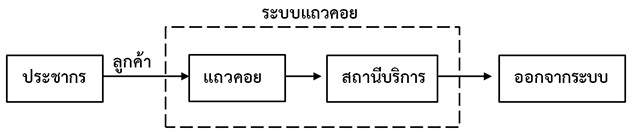
\includegraphics[width=0.75\textwidth]{Query_theory.png}
    \caption{กระบวนการแถวคอย}
    \label{fig:example}
\end{figure}
\indent ในระบบของเรา เรานำแนวคิด Queuing Theory มาประยุกต์ใช้กับการจำลองการเดินทางของผู้โดยสารและการให้บริการโดยรถบัส โดยใช้ Queue Discipline แบบ First in First out และสามารถอธิบายได้ดังนี้
\begin{enumerate}
    \item \textbf{Customers Arrivals (ผู้โดยสารมารอที่ป้าย):} ผู้โดยสารมาถึงป้ายรถตามอัตราการมาถึง (arrival rate) ซึ่งอาจเป็นแบบสุ่มหรือกำหนดเป็นช่วงเวลา
    \item \textbf{Waiting Line (แถวรอขึ้นรถ):} ผู้โดยสารรอรถอยู่ในแถวตามลำดับการมาถึง (FIFO) จนกว่ารถจะมาถึง
    \item \textbf{Server (รถบัส):} รถบัสทำหน้าที่ให้บริการผู้โดยสาร โดยสามารถรับผู้โดยสารได้ตามความจุของรถและเวลาที่ใช้ในการให้บริการ
    \item \textbf{Customer Leaves/Departure (ผู้โดยสารลงจากรถ):} ผู้โดยสารลงจากรถหลังสิ้นสุดการเดินทาง ทำให้พื้นที่ในรถว่างสำหรับผู้โดยสารใหม่
\end{enumerate}

\subsection{Fixed Route Model}
Fixed Route Model คือแบบจำลองการเดินรถโดยที่เส้นทางและเวลาของรถบัสถูกกำหนดตายตัวล่วงหน้า ผู้โดยสารต้องขึ้นรถตามเส้นทางและจุดหยุดที่กำหนดไว้ล่วงหน้า ซึ่งช่วยให้การให้บริการมีความสม่ำเสมอและคาดการณ์ได้ง่าย

\indent ในระบบของเรา Fixed Route Model ถูกใช้สำหรับการจำลองการเดินทางของผู้โดยสารในเส้นทางหลัก เช่น เส้นทางจากต้นทางไปยังปลายทางตามเวลาที่กำหนด โดยรถบัสจะวิ่งตามจุดหยุดที่กำหนด 
ทำให้สามารถวิเคราะห์ความหนาแน่นของผู้โดยสารและเวลารอรถได้

\subsubsection{ประโยชน์}
\begin{itemize}
  \item ช่วยให้ผู้โดยสารรู้เวลารถมาถึงและเส้นทางแน่นอน
  \item ง่ายต่อการวางแผนตารางเวลาและจำนวนรถบัสที่ต้องใช้
  \item สามารถวิเคราะห์ปริมาณผู้โดยสารและปรับปรุงประสิทธิภาพการให้บริการได้ง่าย
\end{itemize}